% !TEX encoding = UTF-8 Unicode

\documentclass[spanish,xcolor=table,svgnames]{beamer}
\definecolor{mediumpurple4}{rgb}{0.36,0.28,0.55}
%colores coporativos
\definecolor{naranja}{rgb}{0.86,0.42,0.06}
\definecolor{gris}{rgb}{0.41,0.41,0.41}
\definecolor{azul}{rgb}{0.06,0.31,0.55}
\definecolor{rojo}{rgb}{1,0,0}
\usecolortheme[named=azul]{structure}

\mode<presentation>
{

  \usetheme{Warsaw}
%\useoutertheme{infolines}
  \setbeamercovered{transparent}
  \setbeamertemplate{navigation symbols}{}
}
\usepackage{listings}
\usepackage{color}
\definecolor{gray97}{gray}{.97}
\definecolor{gray75}{gray}{.75}
\definecolor{gray45}{gray}{.45}
\usepackage{listings}
\lstset{ frame=Ltb,
     framerule=0pt,
     aboveskip=0.5cm,
     framextopmargin=3pt,
     framexbottommargin=3pt,
     framexleftmargin=0.4cm,
     framesep=0pt,
     rulesep=.4pt,
     backgroundcolor=\color{gray97},
     rulesepcolor=\color{black},
     %
     stringstyle=\ttfamily,
     showstringspaces = false,
     basicstyle=\small\ttfamily,
     commentstyle=\color{blue},
     keywordstyle=\bfseries,
     %
     numbers=left,
     numbersep=15pt,
     numberstyle=\tiny,
     numberfirstline = false,
     breaklines=true,
   }
 
% minimizar fragmentado de listados
\lstnewenvironment{listing}[1][]
   {\lstset{#1}\pagebreak[0]}{\pagebreak[0]}
 \lstdefinestyle{consola}
   {basicstyle=\scriptsize\bf\ttfamily,
    backgroundcolor=\color{gray75},
   }
\lstdefinestyle{consola}
   {basicstyle=\scriptsize\bf\ttfamily,
    backgroundcolor=\color{gray75},
   }

\lstdefinestyle{XML}
   {language=XML,
   }

\usepackage[spanish]{babel}
\usepackage[utf8]{inputenc}
\usepackage{charter}
\usepackage[T1]{fontenc}
\usepackage{fancyvrb}
\usepackage{tikz}
%\usepackage{microtype}
\usepackage{xspace}
\usepackage{ctable}
\usepackage{alltt,multicol}

\newcommand{\reduce}{\fontsize{8}{9}\selectfont}
%\usetikzlibrary{chains,positioning,decorations.pathreplacing,fit,scopes}

\title[Gestión de Centro de Mejora del Rendimiento y la Salud]{Gestión de Centro de Mejora del\\Rendimiento y la Salud}
\author[Jesús Soriano Candón]{Jesús Soriano Candón\\Tutora: Lorena Gutiérrez Madroñal}
\institute[UCA]{Ingenierí­a Informática}
\date{15 de diciembre de 2017}

\DefineVerbatimEnvironment{vrbwithcmd}{Verbatim}{commandchars=+(),fontsize=\small}

\begin{document}

\begin{frame}
\vspace*{-3mm}
  \titlepage
  \vspace*{-4mm}
  \begin{figure}
	
\includegraphics[width=0.2\textheight]{logo_uca} 
  \end{figure}
\end{frame}

\frame{\frametitle{͍ndice}\tableofcontents}

%%%%%%%%%%%%%%%%%%%%%%%%%%%%%%%%%
\section{Introducción}
\begin{frame}{Introducción}
    \tableofcontents[currentsection]
\end{frame}

\subsection*{Motivación}
\begin{frame}{Motivación}
  \begin{columns}[onlytextwidth]
    \begin{column}{0.5\textwidth}
      \begin{block}{Motivación del proyecto}
        \begin{itemize}
          \item CoreSport, centro de mejora del rendimiento y la salud.
          \item Necesidad de un sistema telemático de gestión.
          \item Facilitar la gestión a administradores y usuarios.
          \item Necesidad de web pública.
        \end{itemize}
      \end{block}
    \end{column}
    \begin{column}{0.5\textwidth}
      \centering
      \begin{figure}[H]
        \begin{center}
        
\includegraphics[width=0.9\textwidth]{img/coresport.png}
        \end{center}
        \label{fig:logo-coresport}
      \end{figure}
    \end{column}
  \end{columns}
\end{frame}


\subsection*{Alcance}
\begin{frame}{Alcance}
\begin{block}{Objetivos}
Proporcionar una herramienta de gestión completa del centro para los administradores y de actividades y citas para usuarios. \\
Además de la realización de la página web del centro.
\end{block}
\end{frame}



%%%%%%%%%%%%%%%%%%%%%%%%%%%%%%%%%
\section{Planificación}
\frame{\frametitle{Planificación}\tableofcontents[currentsection]}

\subsection*{Metodologí­a}
\begin{frame}{Metodologí­a}
    \begin{center}
    Modelo Incremental
    \begin{figure}[H]
      \begin{center}
          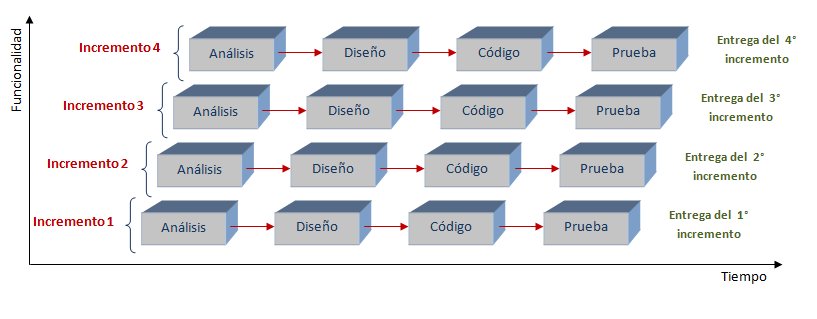
\includegraphics[width=\textwidth]{img/modelo-incremental.png}
      \end{center}
      \label{fig:modelo-incremental}
    \end{figure}
  \end{center}
\end{frame}

\subsection*{Calendario}
\begin{frame}{Calendario}
  \begin{center}
    \begin{figure}[H]
      \begin{center}
          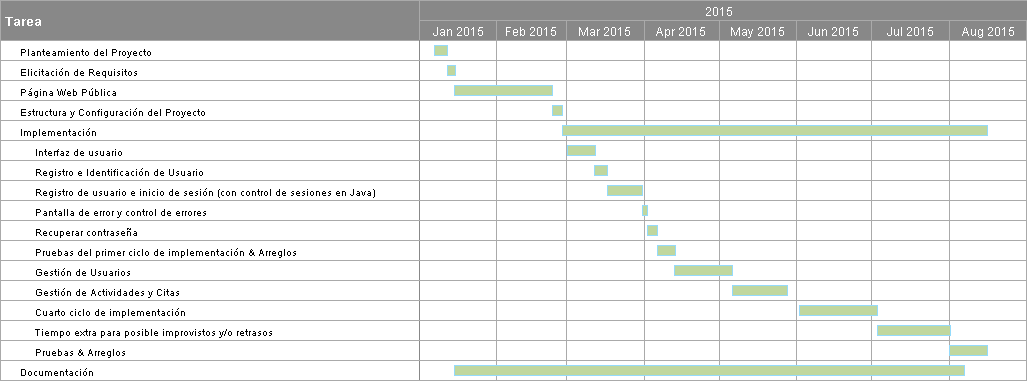
\includegraphics[width=1.0\textwidth]{img/planificacion-gantt.png}
      \end{center}
      \caption{Diagrama de Gantt con tiempos estimados}
      \label{fig:gantt}
    \end{figure}
  \end{center}
\end{frame}


%%%%%%%%%%%%%%%%%%%%%%%%%%%%%%%
\section{Desarrollo del Proyecto}
\frame{\frametitle{Desarrollo del proyecto}\tableofcontents[currentsection]}

\subsection*{Requisitos}
\begin{frame}{Requisitos Funcionales}
  \begin{block}{Requisitos Funcionales}
    \begin{column}{0.5\textwidth}
  \begin{itemize}
    \item Selector de idiomas.
    \item Gestión de datos de usuarios y contraseñas.
    \item Gestión de clases, citas y otros servicios.
    \item Calendario de actividades y citas.
  \end{itemize}
    \end{column}
    \begin{column}{0.5\textwidth}
  \begin{itemize}
    \item Notificaciones.
    \item Registro de operaciones.
    \item Comunicación interna.
    \item *Gestión de usuarios.
    \item *Gestión completa de servicios: Actividades, citas y archivos.
  \end{itemize}
    \end{column}
  \end{block}
  * Requisitos funcionales para administradores.
\end{frame}

\begin{frame}{Requisitos no Funcionales}
  \begin{block}{Requisitos no Funcionales}
  \begin{itemize}
    \item Disponibilidad.
  \begin{itemize}
    \item Adaptabilidad.
  \end{itemize}
    \item Fiabilidad.
    \item Internacionalización.
    \item Usabilidad.
    \item Mantenibilidad.
  \end{itemize}
  \end{block}
\end{frame}



\subsection*{Análisis}
\begin{frame}{Modelo Conceptual}
  \begin{figure}[H]
    \begin{center}
        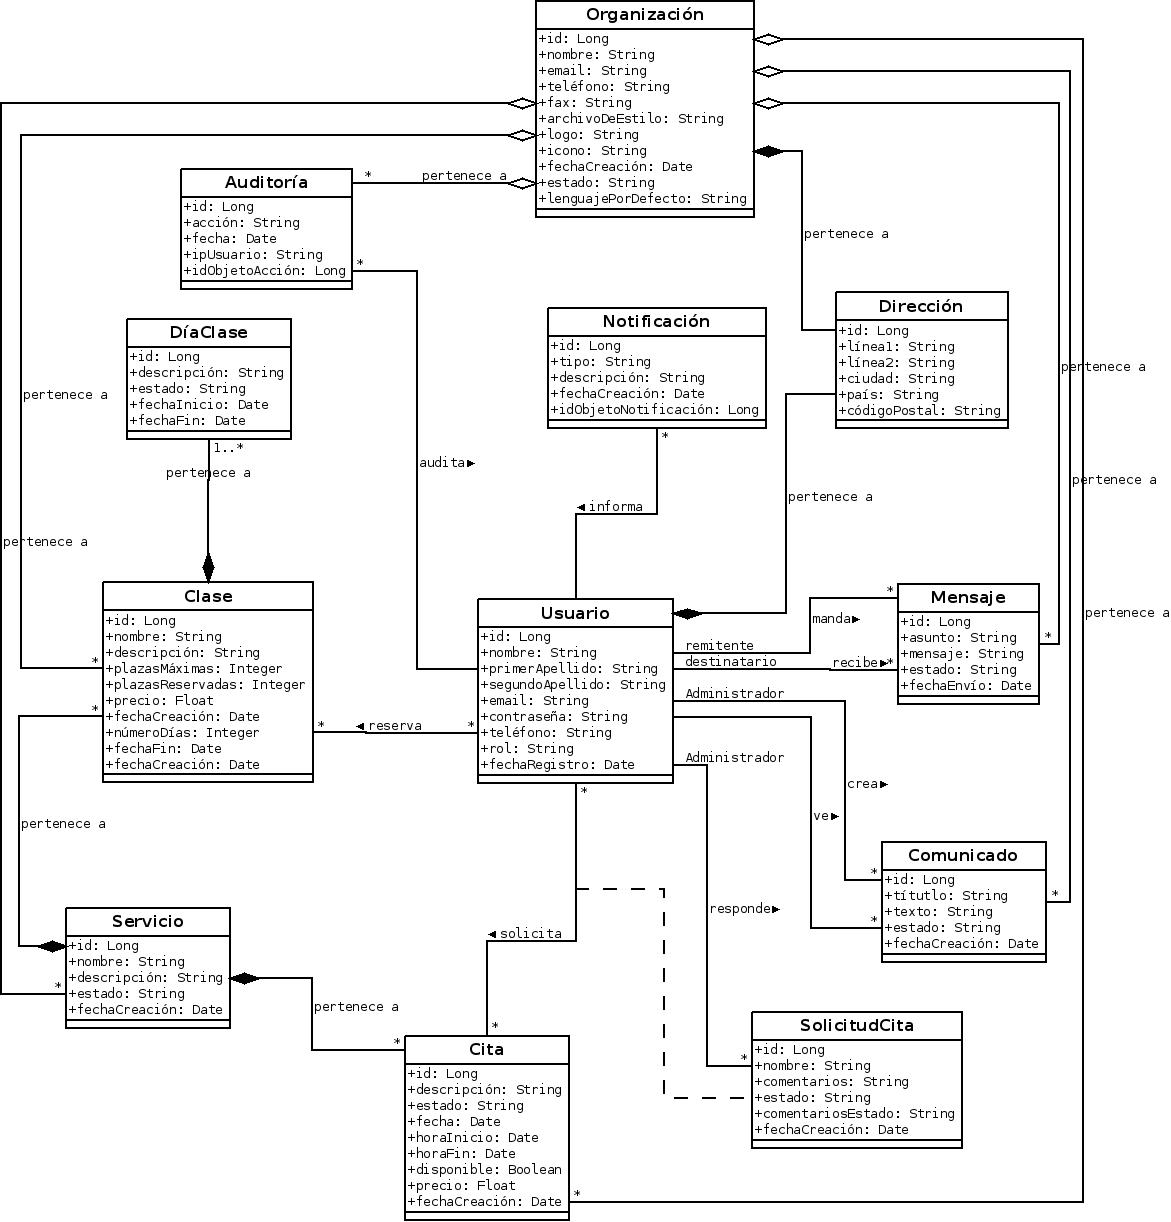
\includegraphics[width=0.85\textwidth]{img/modelo-conceptual.jpeg}
    \end{center}
    \label{fig:conceptual}
\end{figure}
\end{frame}


\subsection*{Diseño}
\begin{frame}{Diseño de Interfaz de Usuario}
  \begin{figure}[H]
    \begin{center}
        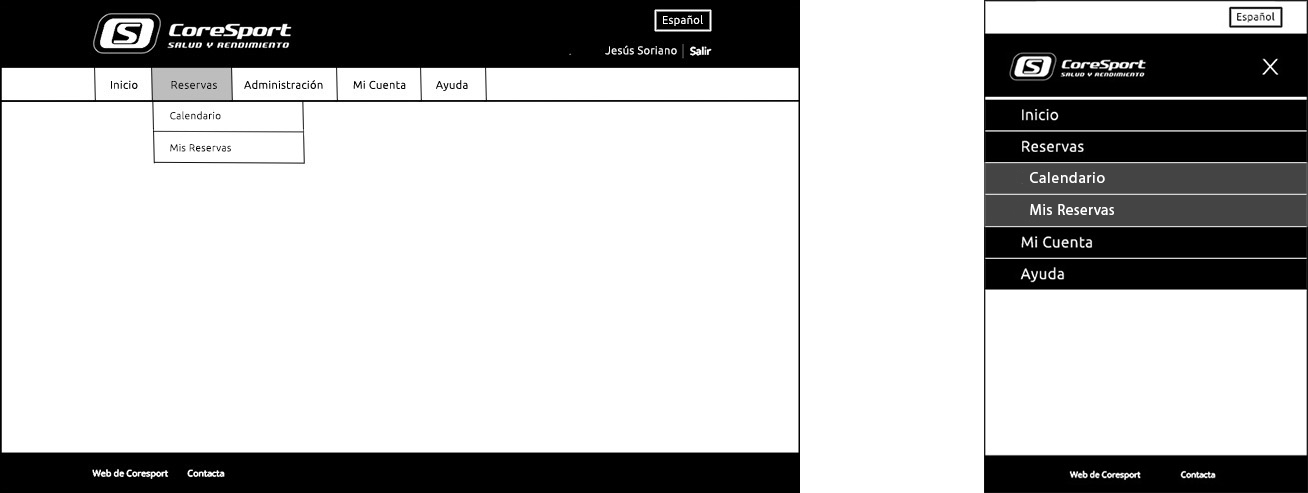
\includegraphics[width=0.7\textwidth]{img/comparativa-interfaces.png}
    \end{center}
      \caption{Diseño adaptable (responsive)}
    \label{fig:responsive}
\end{figure}
\end{frame}

\begin{frame}{Diseño de Interfaz de Usuario}
  \begin{figure}[H]
    \begin{center}
      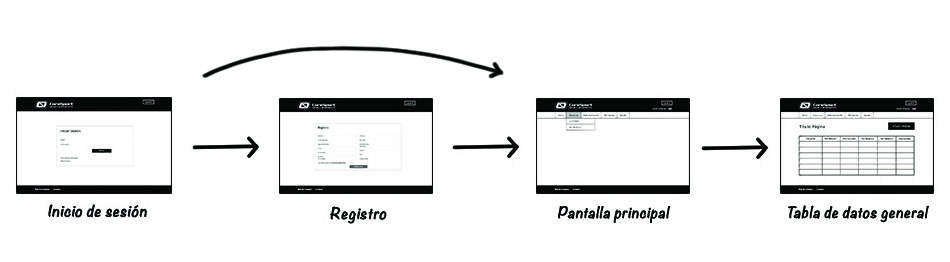
\includegraphics[width=1.0\textwidth]{img/navegacion.jpg}
    \end{center}
      \caption{Navegación}
    \label{fig:navegacion}
\end{figure}
\end{frame}





\subsection*{Implementación}

\begin{frame}{Entorno Tecnológico}
  \begin{figure}[H]
    \begin{center}
        
\includegraphics[width=0.75\textwidth]{img/logos-combinados.jpg}
    \end{center}
    \label{fig:tecnologias}
  \end{figure}
\end{frame}

\begin{frame}{Entorno Tecnológico}
  \begin{figure}[H]
    \begin{center}
        
\includegraphics[width=0.75\textwidth]{img/logos-combinados-java.jpg}
    \end{center}
    \label{fig:tecnologias-java}
  \end{figure}
\end{frame}

\begin{frame}{Entorno Tecnológico}
  \begin{figure}[H]
    \begin{center}
        
\includegraphics[width=0.75\textwidth]{img/logos-combinados-postgresql.jpg}
    \end{center}
    \label{fig:tecnologias-bd}
  \end{figure}
\end{frame}

\begin{frame}{Entorno Tecnológico}
  \begin{figure}[H]
    \begin{center}
        
\includegraphics[width=0.75\textwidth]{img/logos-combinados-frontend.jpg}
    \end{center}
    \label{fig:tecnologias-frontend}
  \end{figure}
\end{frame}

\begin{frame}{Entorno Tecnológico}
  \begin{figure}[H]
    \begin{center}
        
\includegraphics[width=0.75\textwidth]{img/logos-combinados-latex.jpg}
    \end{center}
    \label{fig:tecnologias-latex}
  \end{figure}
\end{frame}

\begin{frame}{Entorno Tecnológico}
  \begin{figure}[H]
    \begin{center}
        
\includegraphics[width=0.75\textwidth]{img/logos-combinados-git.jpg}
    \end{center}
    \label{fig:tecnologias-git}
  \end{figure}
\end{frame}


\begin{frame}{Entorno Tecnológico}
  \begin{figure}[H]
    \begin{center}
        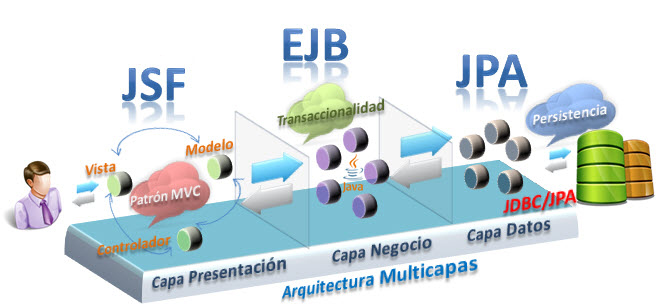
\includegraphics[width=0.75\textwidth]{img/arquitectura-jee.jpg}
    \end{center}
      \caption{Arquitectura multicapas con frameworks}
    \label{fig:arquitectura-jee}
  \end{figure}
\end{frame}


\begin{frame}{Estructura de Ficheros}
  \begin{columns}[onlytextwidth]
    \begin{column}{0.5\textwidth}
      \centering
      \begin{figure}[H]
        \begin{center}
        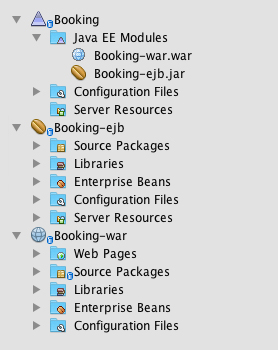
\includegraphics[width=0.7\textwidth]{img/estructura-ficheros.jpg}
        \end{center}
        \caption{Estructura de ficheros}
        \label{fig:estructura-proyecto}
      \end{figure}
    \end{column}
    \begin{column}{0.5\textwidth}
    \end{column}
  \end{columns}
\end{frame}

\begin{frame}{Estructura de Ficheros}
  \begin{columns}[onlytextwidth]
    \begin{column}{0.5\textwidth}
      \centering
      \begin{figure}[H]
        \begin{center}
        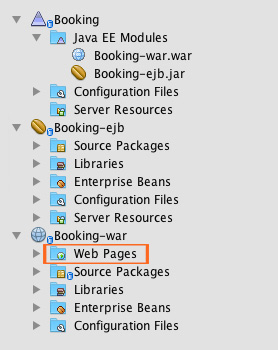
\includegraphics[width=0.7\textwidth]{img/estructura-ficheros-web.jpg}
        \end{center}
        \caption{Estructura de ficheros}
        \label{fig:estructura-proyecto}
      \end{figure}
    \end{column}
    \begin{column}{0.5\textwidth}
      \centering
      \begin{figure}[H]
        \begin{center}
        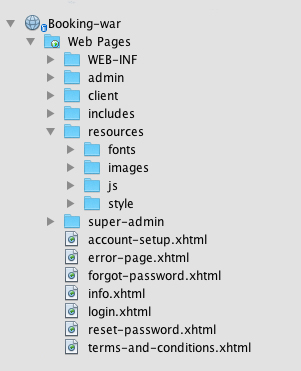
\includegraphics[width=0.7\textwidth]{img/web-pages.jpg}
        \end{center}
        \caption{Directorio Web Pages}
        \label{fig:estructura-web}
      \end{figure}
    \end{column}
  \end{columns}
\end{frame}


\begin{frame}{web.xml}
  \begin{figure}[H]
    \begin{center}
        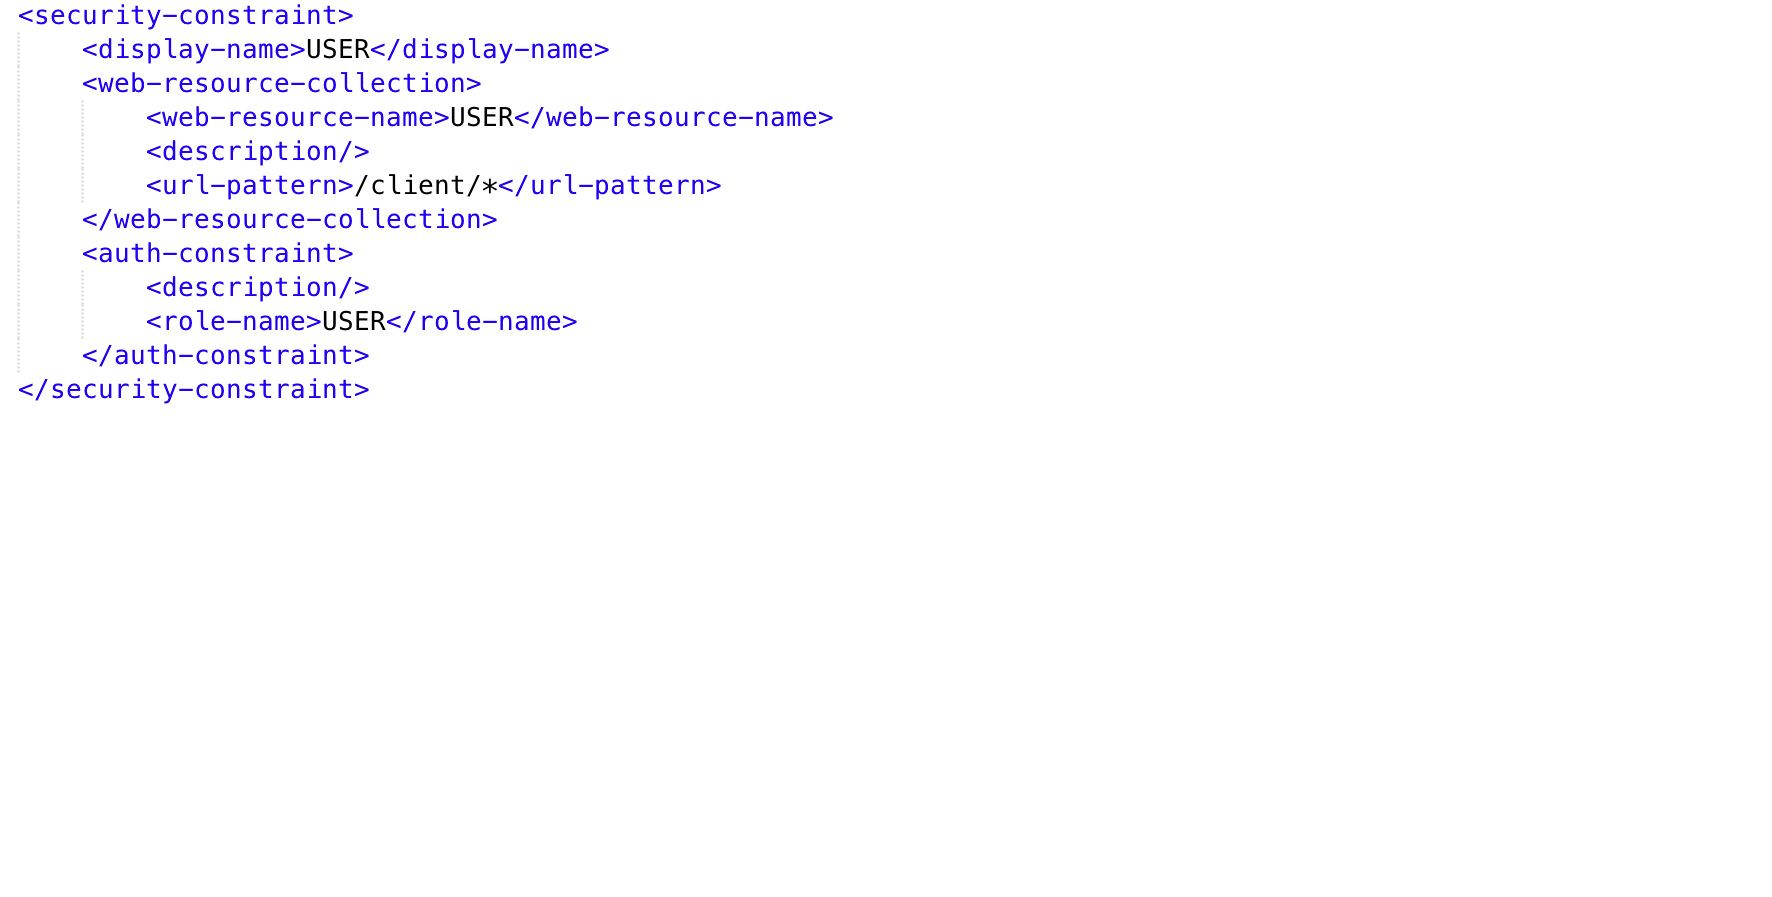
\includegraphics[width=\textwidth]{img/web-xml-client.jpg}
    \end{center}
    \label{fig:web-xml-client}
  \end{figure}
\end{frame}

\begin{frame}{web.xml}
  \begin{figure}[H]
    \begin{center}
        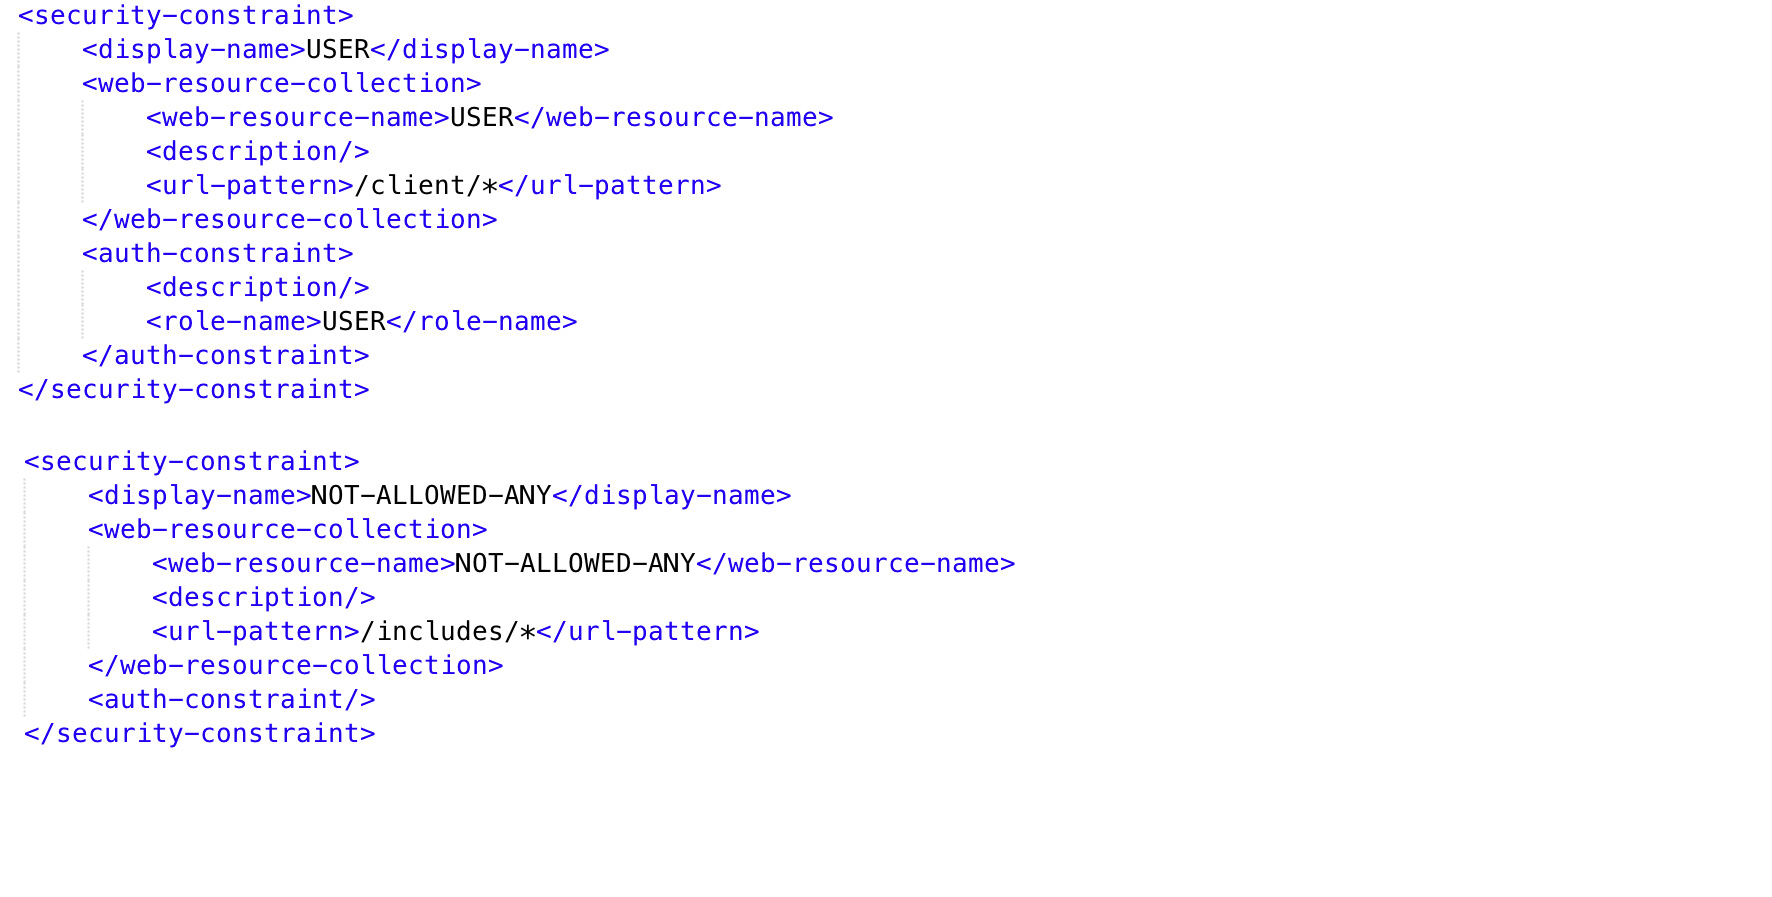
\includegraphics[width=\textwidth]{img/web-xml-includes.jpg}
    \end{center}
    \label{fig:web-xml-includes}
  \end{figure}
\end{frame}

\begin{frame}{web.xml}
  \begin{figure}[H]
    \begin{center}
        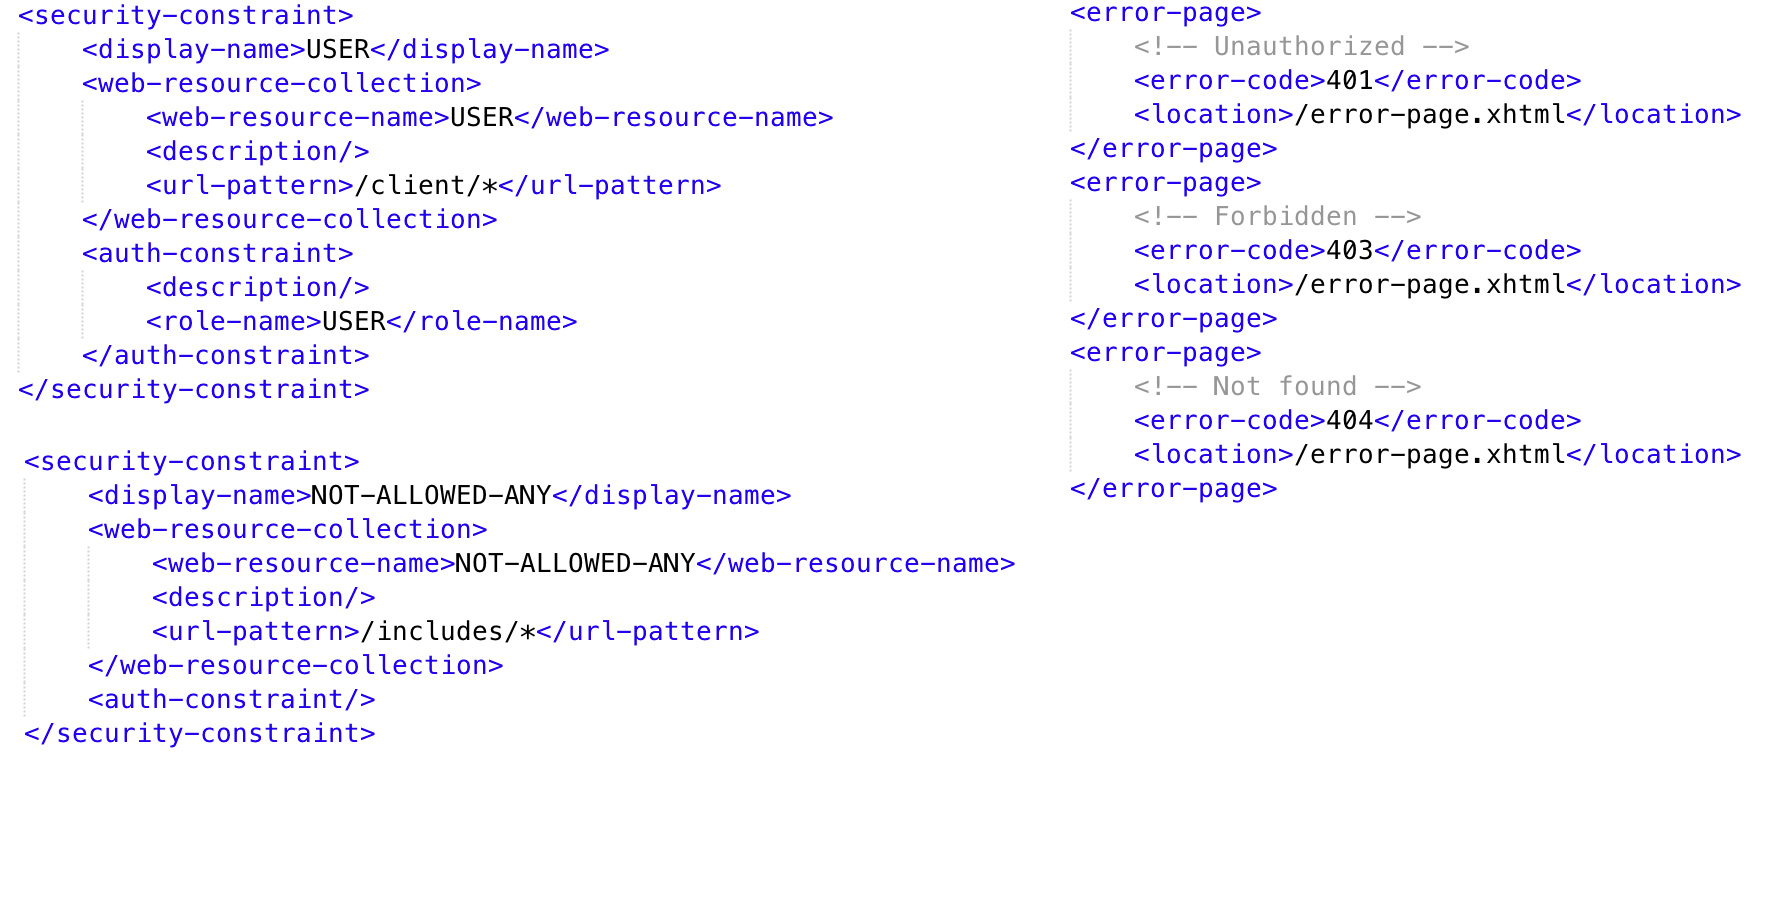
\includegraphics[width=\textwidth]{img/web-xml-errores.jpg}
    \end{center}
    \label{fig:web-xml-errores}
  \end{figure}
\end{frame}

\begin{frame}{web.xml}
  \begin{figure}[H]
    \begin{center}
        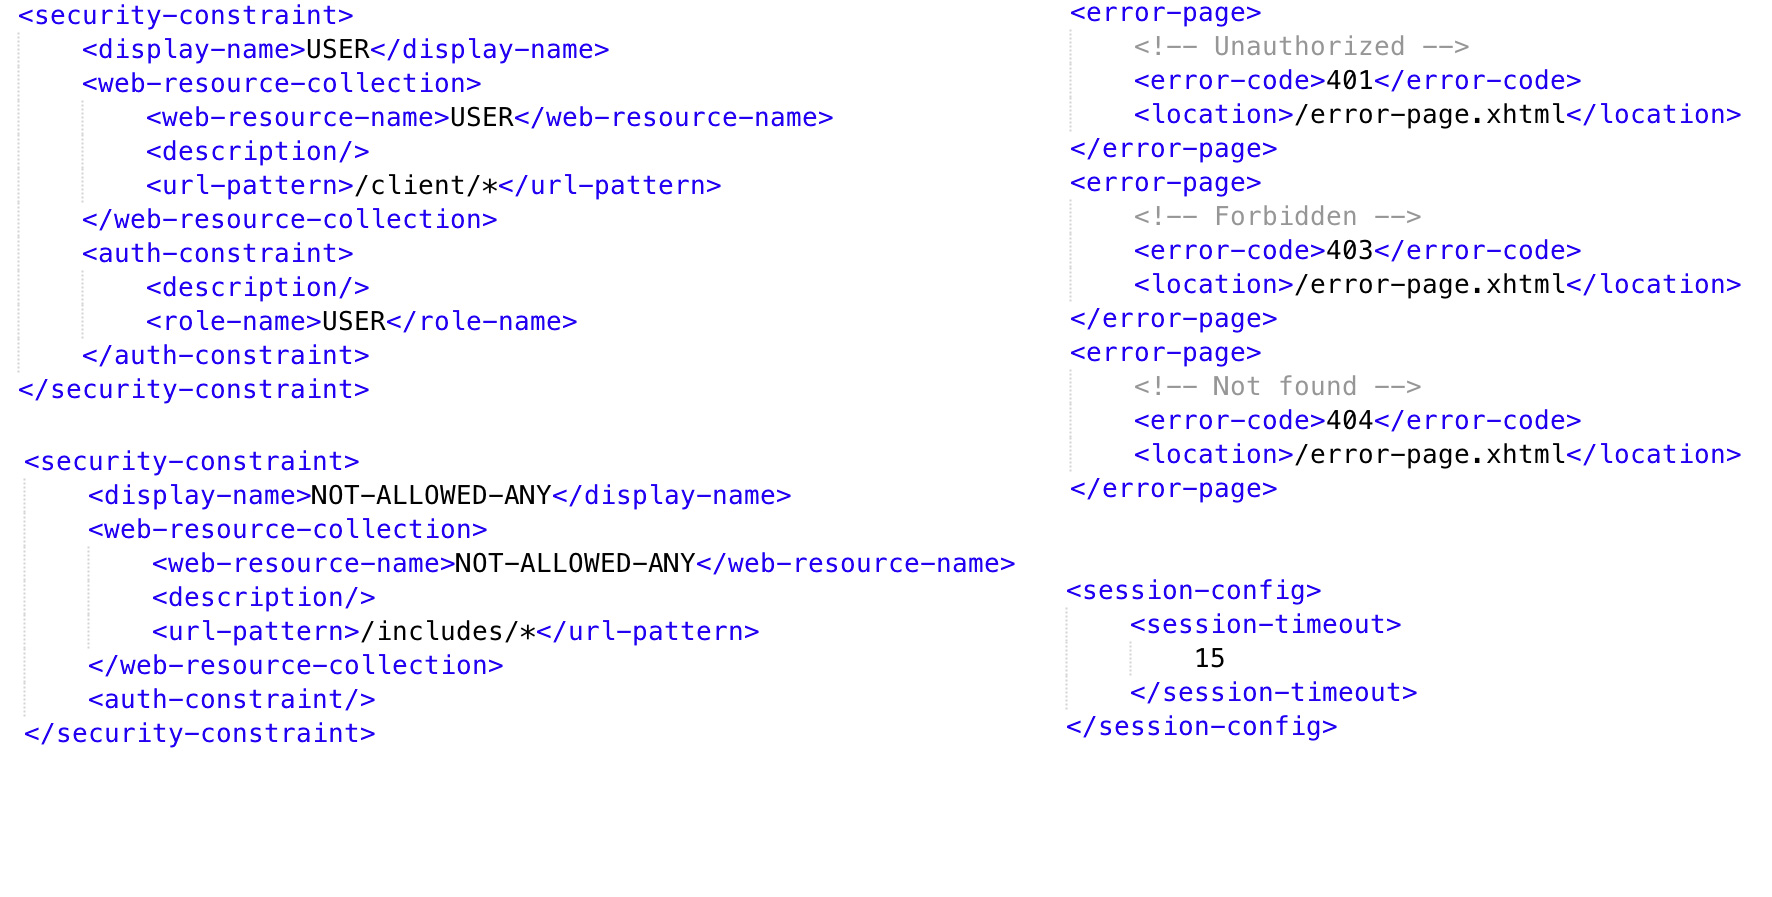
\includegraphics[width=\textwidth]{img/web-xml-sesion.jpg}
    \end{center}
    \label{fig:web-xml-sesion}
  \end{figure}
\end{frame}

\begin{frame}{web.xml}
  \begin{figure}[H]
    \begin{center}
        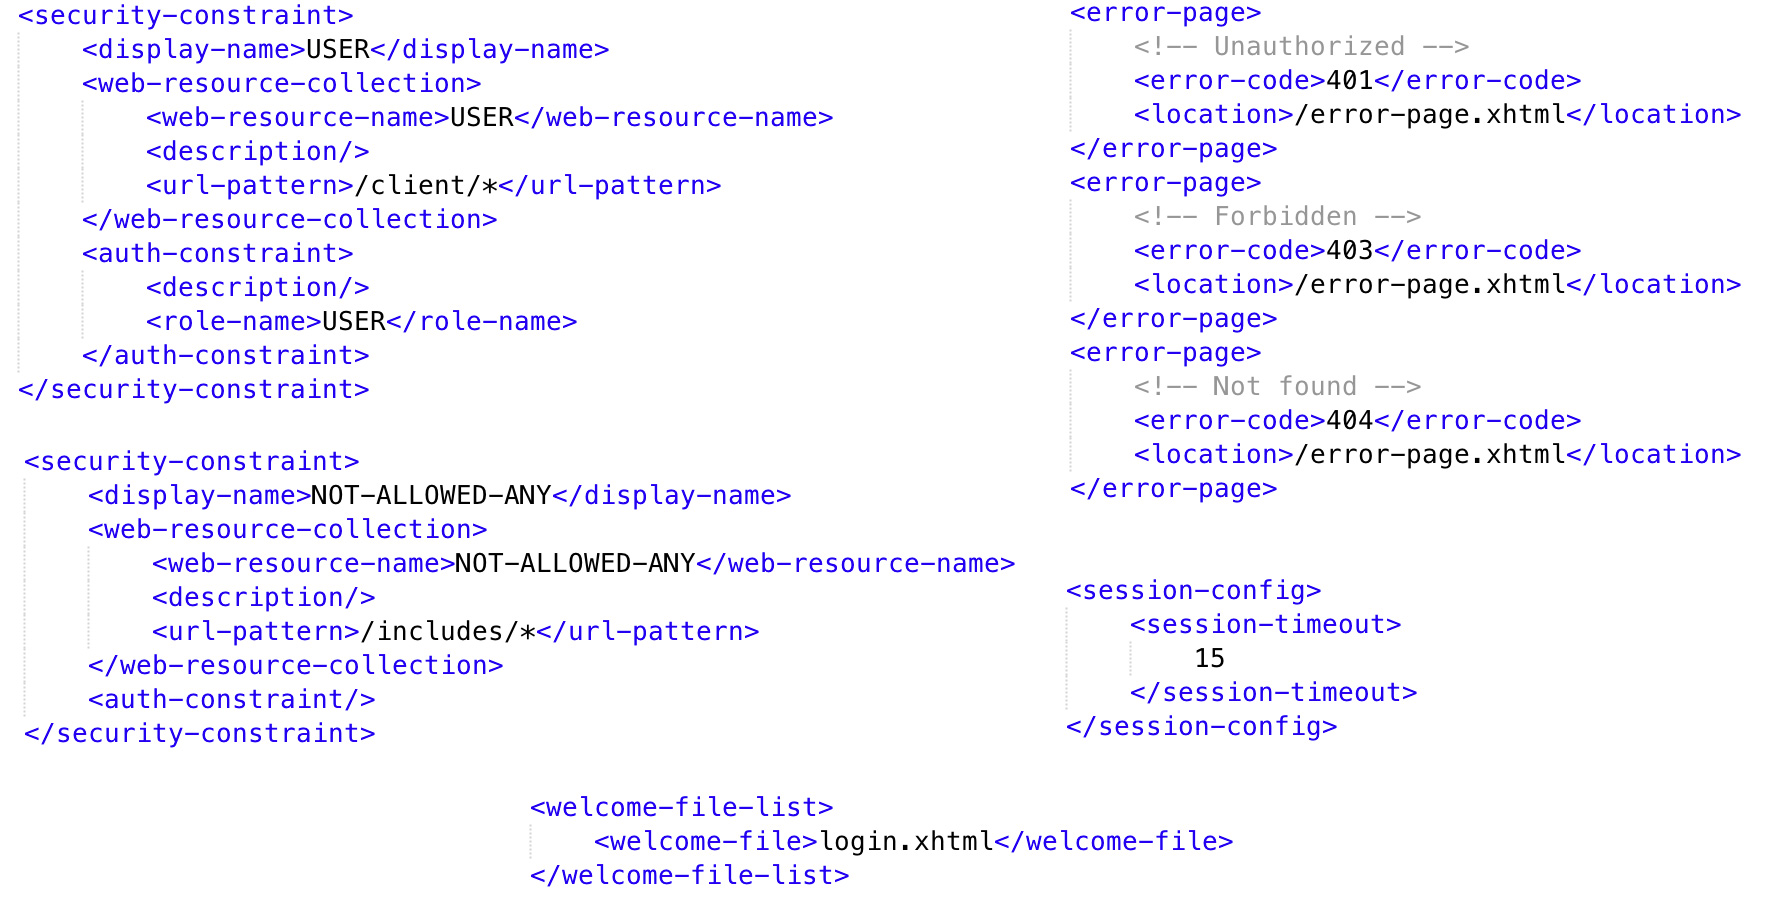
\includegraphics[width=\textwidth]{img/web-xml-login.jpg}
    \end{center}
    \label{fig:web-xml-login}
  \end{figure}
\end{frame}


\begin{frame}{Estructura de Ficheros}
  \begin{columns}[onlytextwidth]
    \begin{column}{0.5\textwidth}
      \centering
      \begin{figure}[H]
        \begin{center}
        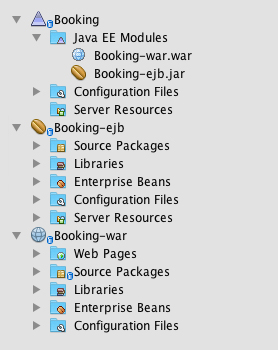
\includegraphics[width=0.7\textwidth]{img/estructura-ficheros.jpg}
        \end{center}
        \caption{Estructura de ficheros}
        \label{fig:estructura-proyecto-3}
      \end{figure}
    \end{column}
    \begin{column}{0.5\textwidth}
    \end{column}
  \end{columns}
\end{frame}

\begin{frame}{Estructura de Ficheros}
  \begin{columns}[onlytextwidth]
    \begin{column}{0.5\textwidth}
      \centering
      \begin{figure}[H]
        \begin{center}
        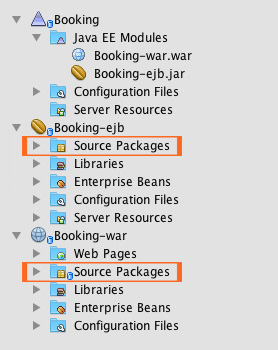
\includegraphics[width=0.7\textwidth]{img/estructura-ficheros-war-ejb-sources.jpg}
        \end{center}
        \caption{Estructura de ficheros}
        \label{fig:estructura-proyecto-4}
      \end{figure}
    \end{column}
    \begin{column}{0.5\textwidth}
      \centering
      \begin{figure}[H]
        \begin{center}
        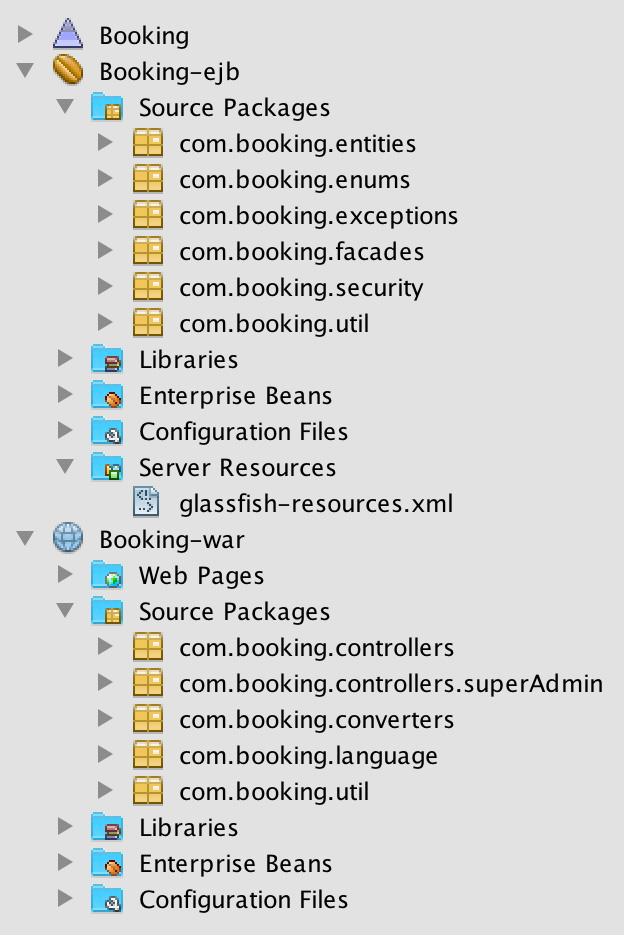
\includegraphics[width=0.7\textwidth]{img/estructura-ficheros-war-ejb-sources-abierto.jpg}
        \end{center}
        \label{fig:estructura-web}
      \end{figure}
    \end{column}
  \end{columns}
\end{frame}


\begin{frame}{Comunicación por Capas. Ejemplo.}
  \begin{figure}[H]
    \begin{center}
        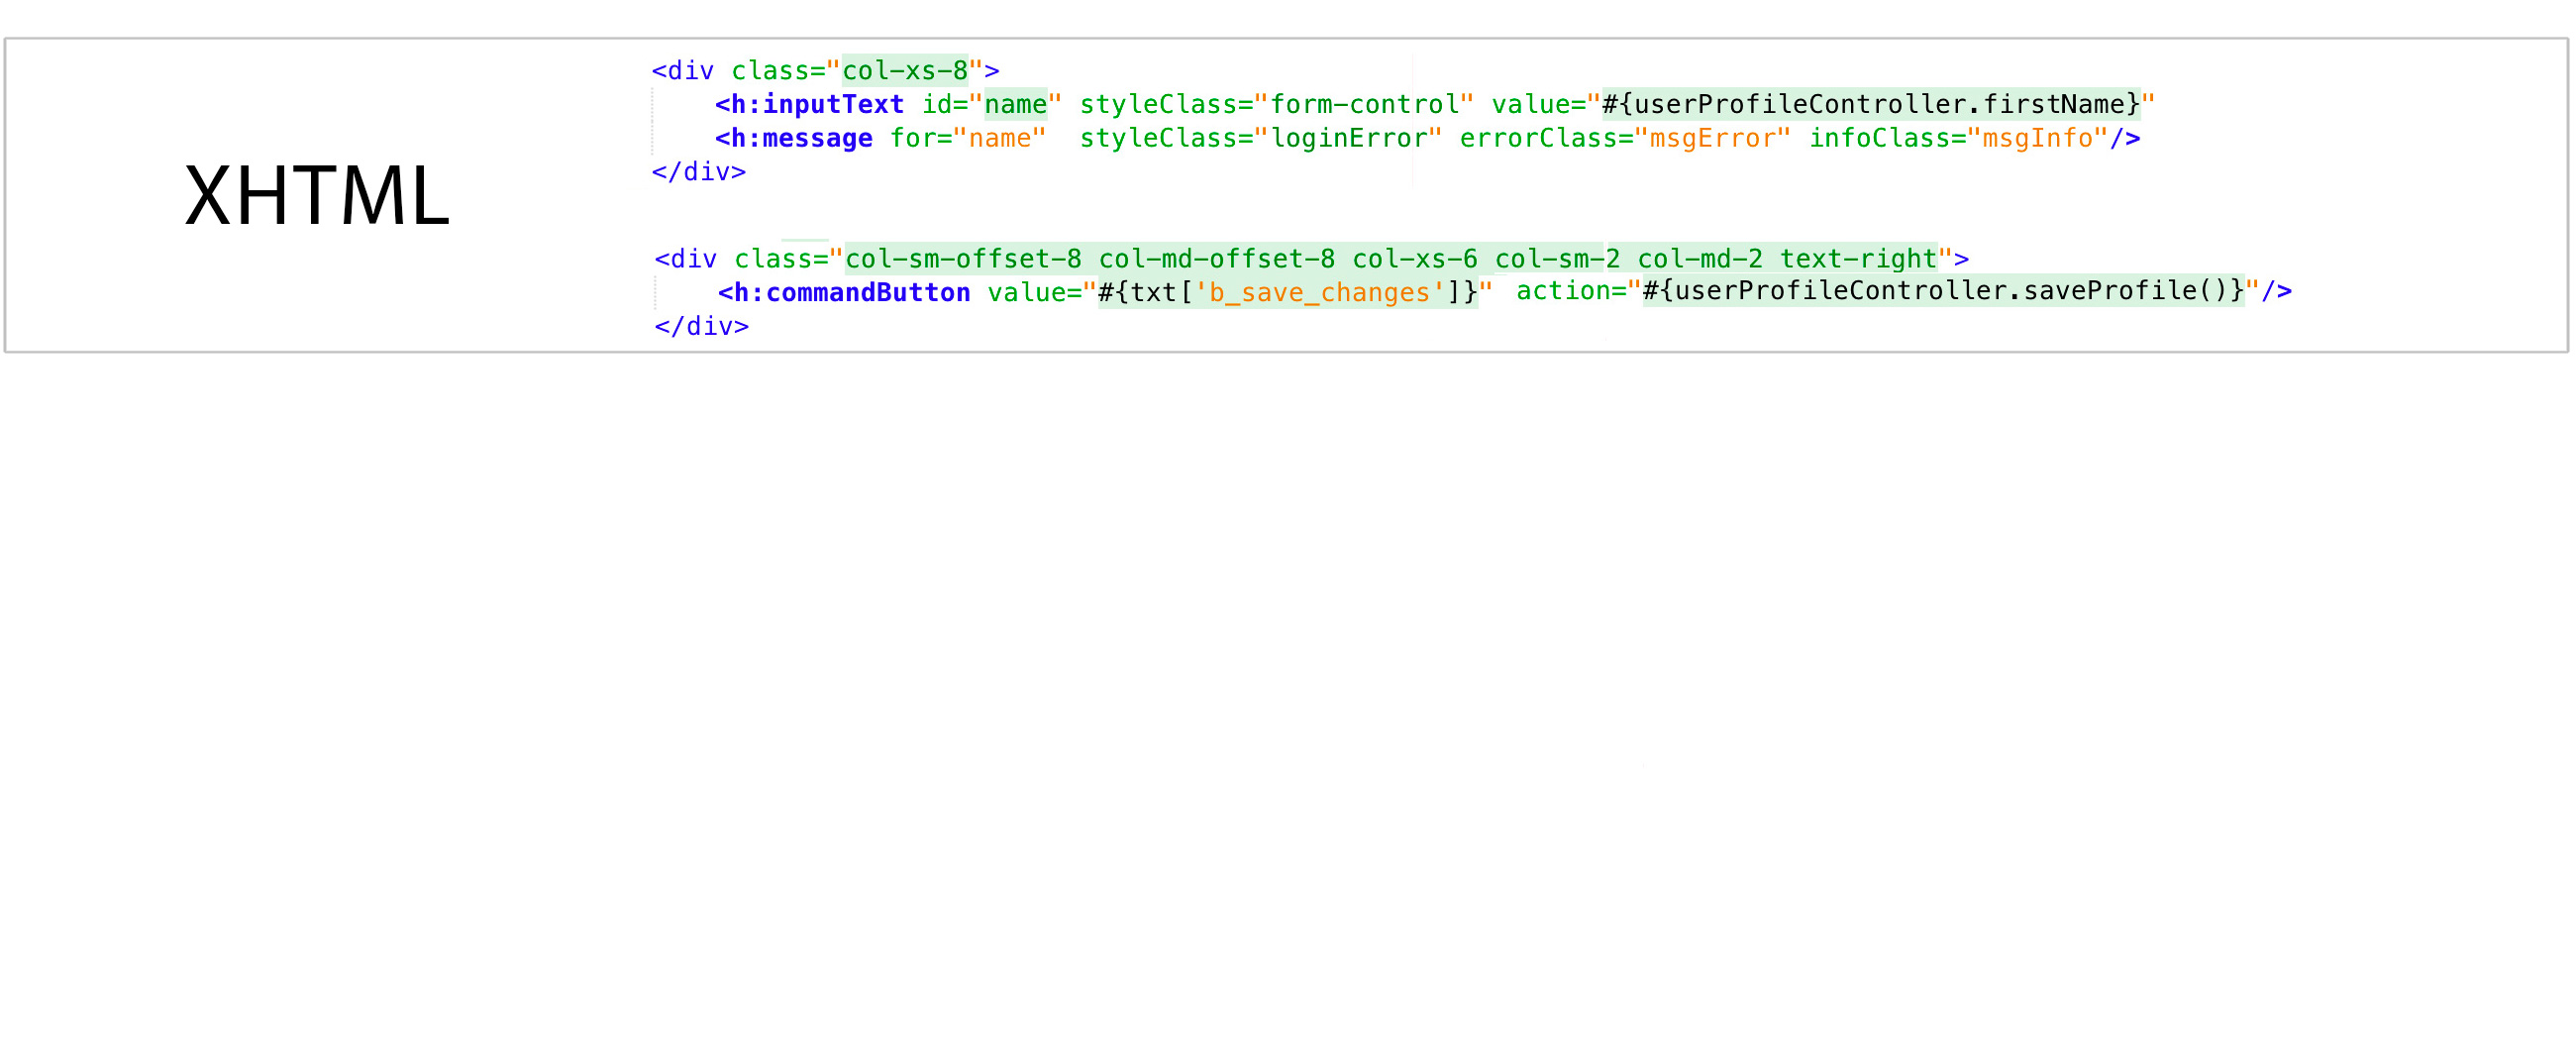
\includegraphics[width=\textwidth]{img/comunicacion-ficheros-xhtml.jpg}
    \end{center}
    \label{fig:comunicacion-ficheros-xhtml}
  \end{figure}
\end{frame}

\begin{frame}{Comunicación por Capas. Ejemplo.}
  \begin{figure}[H]
    \begin{center}
        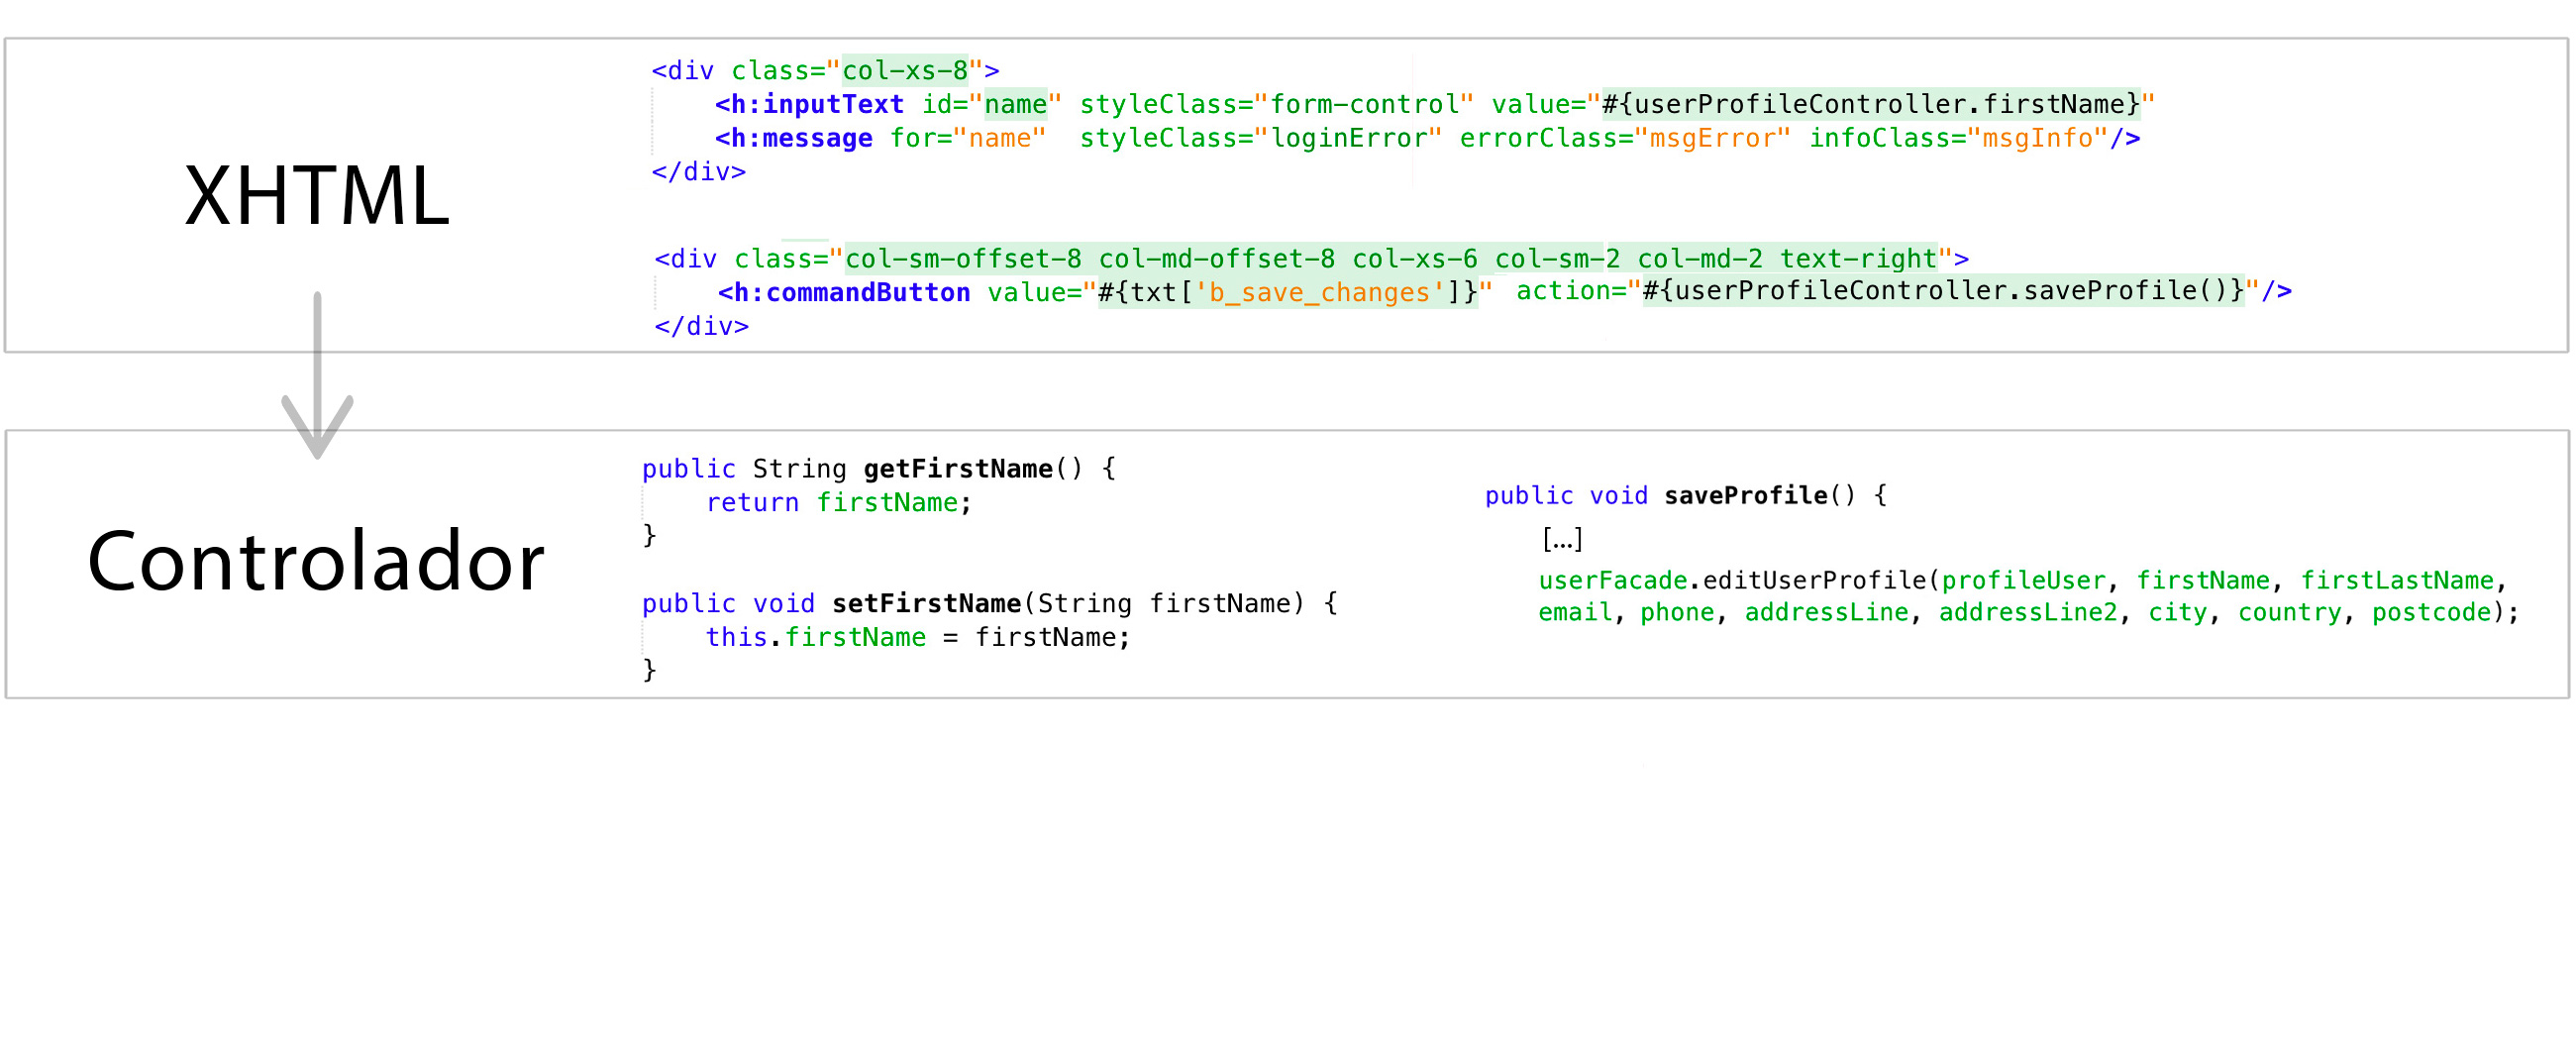
\includegraphics[width=\textwidth]{img/comunicacion-ficheros-controlador.jpg}
    \end{center}
    \label{fig:comunicacion-ficheros-controlador}
  \end{figure}
\end{frame}

\begin{frame}{Comunicación por Capas. Ejemplo.}
  \begin{figure}[H]
    \begin{center}
        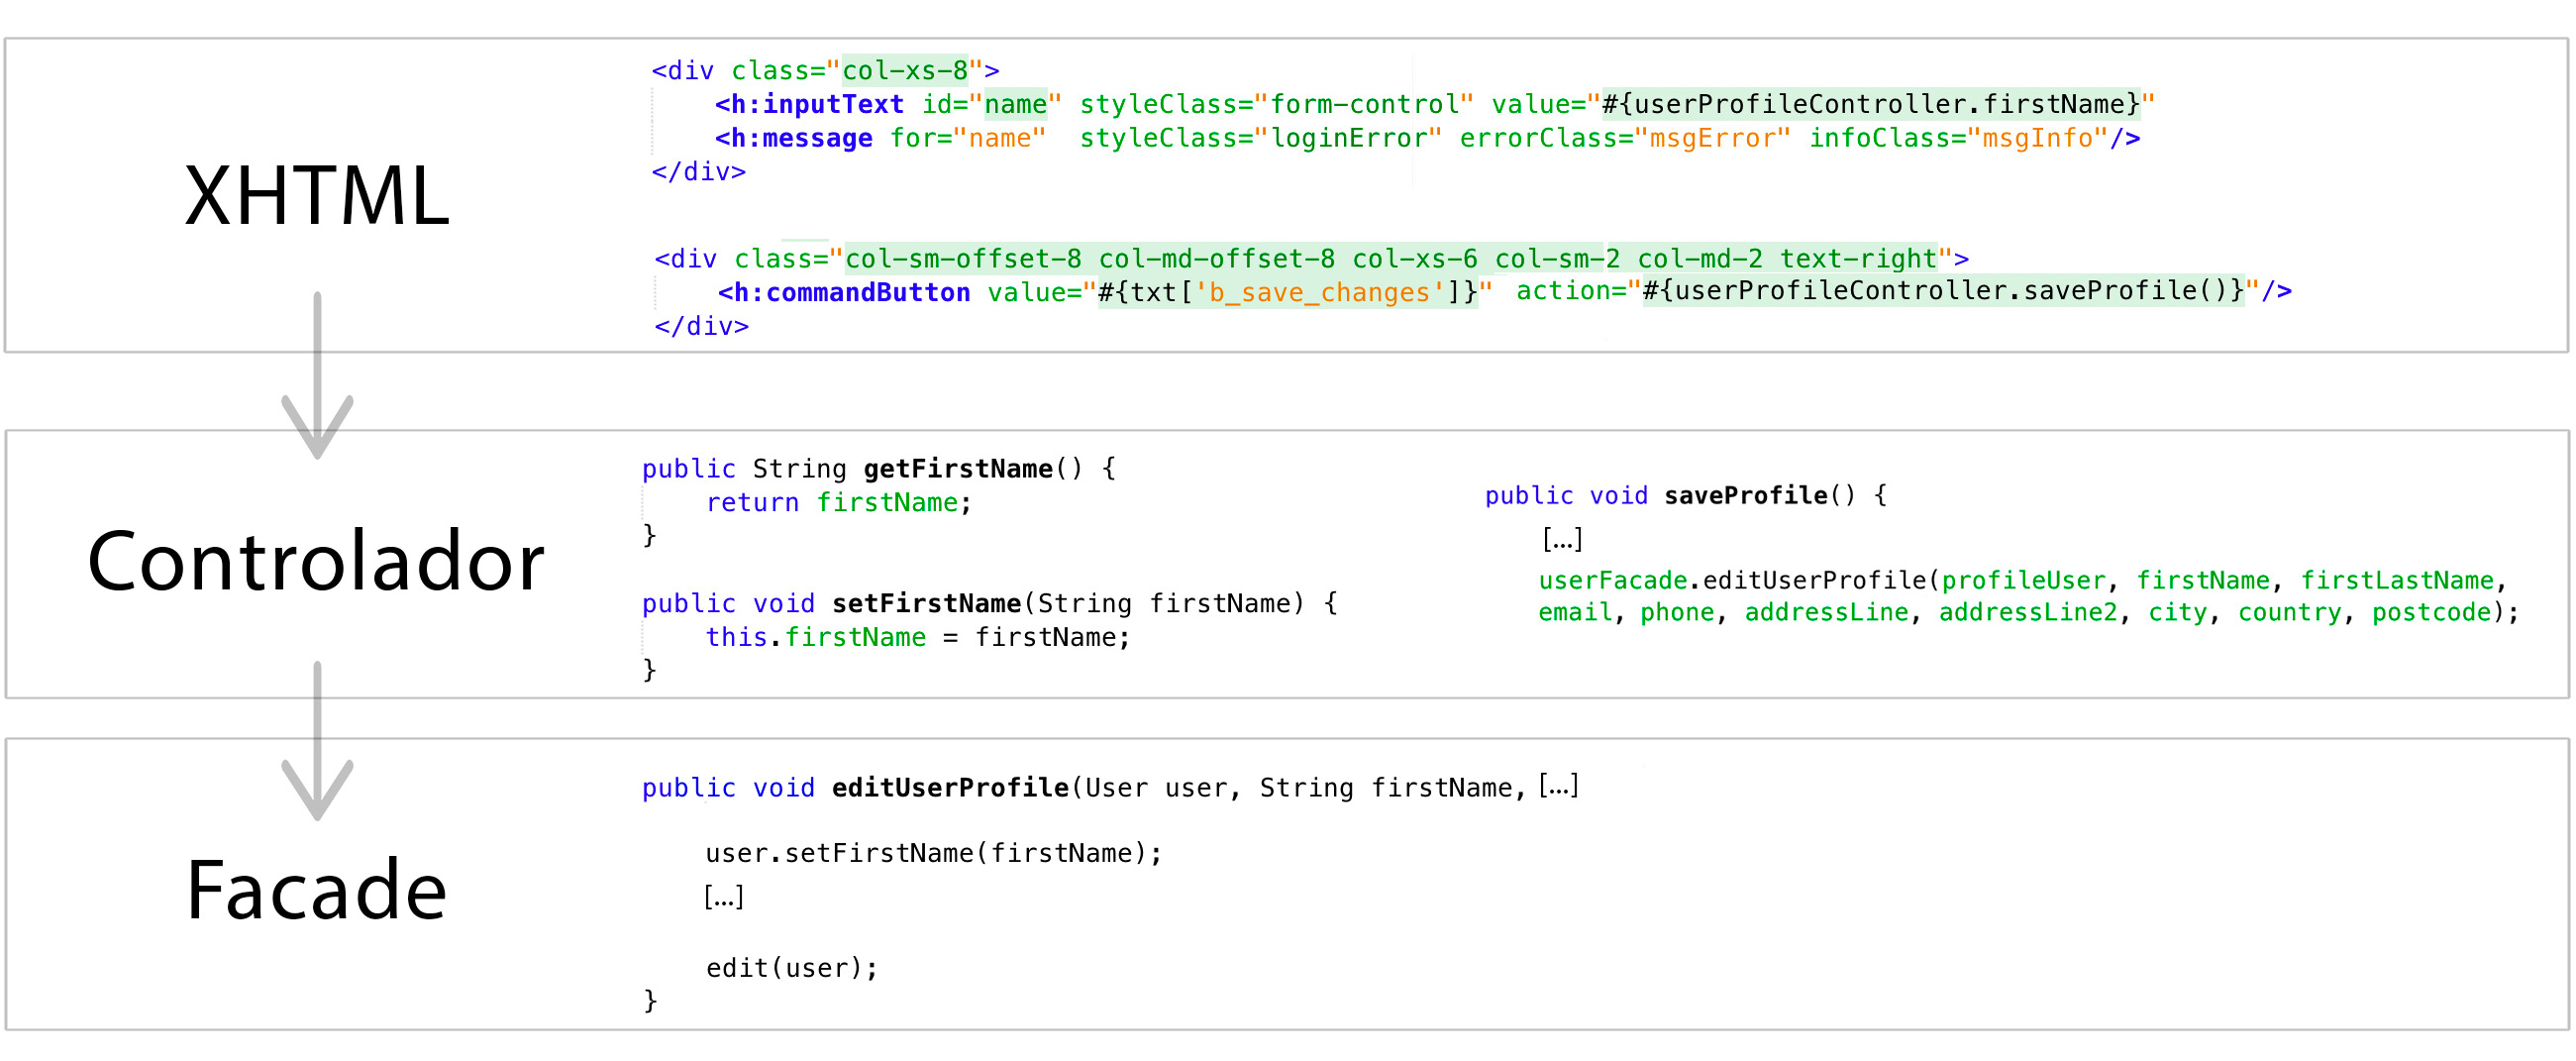
\includegraphics[width=\textwidth]{img/comunicacion-ficheros-facade.jpg}
    \end{center}
    \label{fig:comunicacion-ficheros-facade}
  \end{figure}
\end{frame}



\begin{frame}{Pruebas}
  \begin{block}{Niveles de Pruebas}
    \begin{itemize}
      \item Pruebas unitarias.
      \item Pruebas de integración.
      \item Pruebas de sistema:
      \begin{itemize}
        \item Pruebas funcionales.
        \item Pruebas no funcionales.
      \end{itemize}
      \item Siguiente: Pruebas en entrono real.
  \end{itemize}
  \end{block}
\end{frame}




%%%%%%%%%%%%%%%%%%%%%%%%%%%%%%%
\section{Conclusiones}
\frame{\frametitle{Conclusiones}\tableofcontents[currentsection]}

\subsection*{Objetivos alcanzados}
\begin{frame}{Objetivos alcanzados}
\begin{block}{¿Qué se ha logrado?}
  \begin{itemize}
    \item La aplicación resultado del desarrollo del proyecto es capaz de satisfacer los requisitos tanto funcionales como no funcionales establecidos:
  \begin{itemize}
    \item Gestión de citas y actividades para usuarios.
    \item Gestión completa para administradores.
  \end{itemize}
    \item Página web pública: www.coresport.es. Cumpliendo la necesidad de la empresa.
  \end{itemize}
\end{block}
\end{frame}

\subsection*{Lecciones aprendidas}
\begin{frame}{Lecciones aprendidas}
\begin{block}{Valoración}
  \begin{itemize}
    \item Se han mejorado los conocimientos tanto de Java y los frameworks usados, como de base de datos, \LaTeX, control de versiones, etc.
    \item Importancia de seguir una metodología de software y realización de planificación, análisis y diseño previos a la implementación.
    \item Trato con el cliente.
    \item Resolución de problemas, autoaprendizaje y gestión del tiempo.
  \end{itemize}
\end{block}
\end{frame}

\subsection*{Trabajo futuro}
\begin{frame}{Trabajo futuro}
\begin{block}{Trabajos futuros}
\begin{itemize}
\item Clases o citas recursivas.
\item Segmentación de usuarios.
\item Notificaciones y permisos.
\item Web pública: internacionalización, blog y mejoras.
\end{itemize}
\end{block}
\end{frame}

\section{Bibliografí­a}
\begin{frame}{Bibliografí­a}
  \tableofcontents[currentsection]
\end{frame}

\begin{frame}{Bibliografí­a}
  \begin{thebibliography}{10}
    \beamertemplatebookbibitems
    \bibitem{1} Bert Bates y Kathy Sierra. Head First EJB. O'Reilly Media, Junio 2009.
    \bibitem{2} Oracle. \emph{Introduction to the Java Persistence API, The Java EE 6 Tutorial}. docs.oracle.com/javaee/6/tutorial/doc/bnbpz.html.
    \bibitem{3} Web Oficial PrimeFaces. www.primefaces.org.
    \bibitem{4} Web Oficial PostgreSQL. www.postgresql.org.
    \bibitem{5} Wikipedia. \emph{Programación por Capas}. es.wikipedia.org/wiki/Programación\_por\_capas.
  \end{thebibliography} 
\end{frame}

\begin{frame}{Bibliografí­a}
  \begin{thebibliography}{10}
    \beamertemplatebookbibitems
    \bibitem{6} Universidad de Alicante. \emph{Introducción a JavaServer Faces}. www.jtech.ua.es/j2ee/publico/jsf-2012-13/sesion01-apuntes.html.
    \bibitem{7} Universidad de Alicante. \emph{Introducción a la Tecnología EJB. www.jtech.ua.es/j2ee/2003-2004/abierto-j2ee-2003-2004/ejb/sesion01-apuntes.htm}.
    \bibitem{8} Universidad de Alicante. \emph{El MVC en JavaServer Faces}. www.jtech.ua.es/j2ee/publico/jsf-2012-13/sesion02-apuntes.html.
    \bibitem{9} Web de GoJava. \emph{JDBC security realm with glassfish and jsf}. jugojava.blogspot.com.es/2011/02/jdbc-security-realm-with-glassfish-and.html
  \end{thebibliography} 
\end{frame}




%%%%%%%%%%%%%%%%%%%%%%%%%%%%%%%
\section{Demostración}
\begin{frame}{Demostración}
  \tableofcontents[currentsection]
\end{frame}





\appendix
\frame
{
  \begin{center}
    \Huge{Gracias por su atención}
  \end{center}
  \begin{center}
    \url{www.github.com/JesusSoriano/gestor-reservas}
  \end{center}
}
\end{document}